\documentclass{article}
\usepackage[utf8]{inputenc}
\usepackage{titling}
\usepackage{graphicx}
\usepackage{xcolor}
\usepackage[colorlinks=true,linkcolor=darkgray, urlcolor =gray]{hyperref}
\usepackage[spanish]{babel}
\DeclareUnicodeCharacter{301}{~}
\usepackage{url}
\DeclareUnicodeCharacter{202F}{\,}


\title{Práctica	LTE. Análisis de protocolos LTE	en la Interfaz S1}
\author{Cristina Díaz García}
\date{Enero 2019}

\renewcommand\maketitlehooka{\null\mbox{}\vfill}
\renewcommand\maketitlehookd{\vfill\null}


\begin{document}

\addcontentsline{toc}{section}{Índice general}

\begin{titlingpage}
\maketitle

\begin{center}
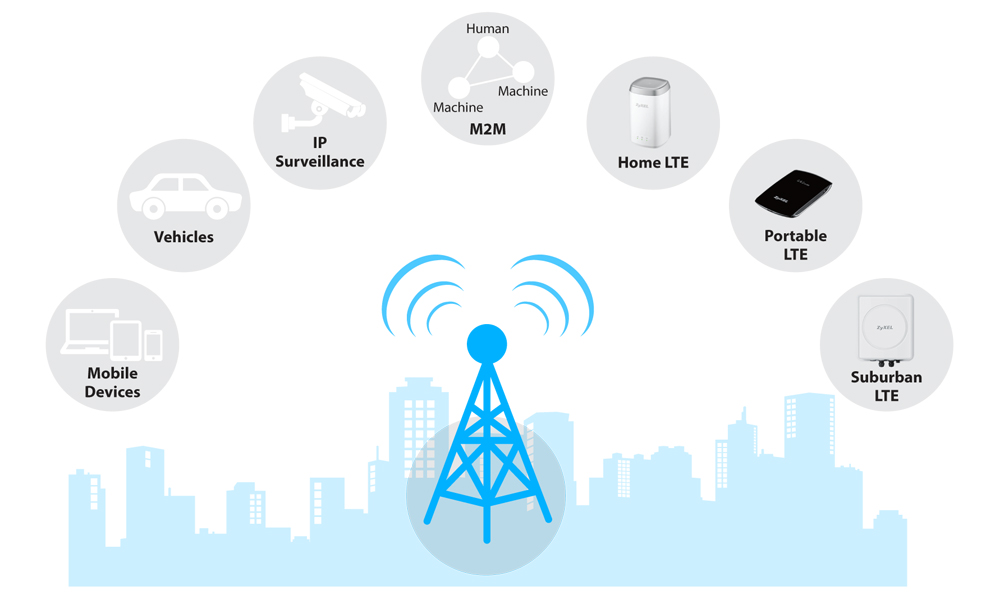
\includegraphics[scale=1.5]{images/lte.jpg} 
\end{center}

\end{titlingpage}

\newpage

\tableofcontents

\newpage

\section{Ejercicio 1. Traza S1.pcap}

\textbf{a) ¿Qué tipo de tráfico contiene la traza, qué está ocurriendo?}

Una llamada telefónica.

\begin{center}
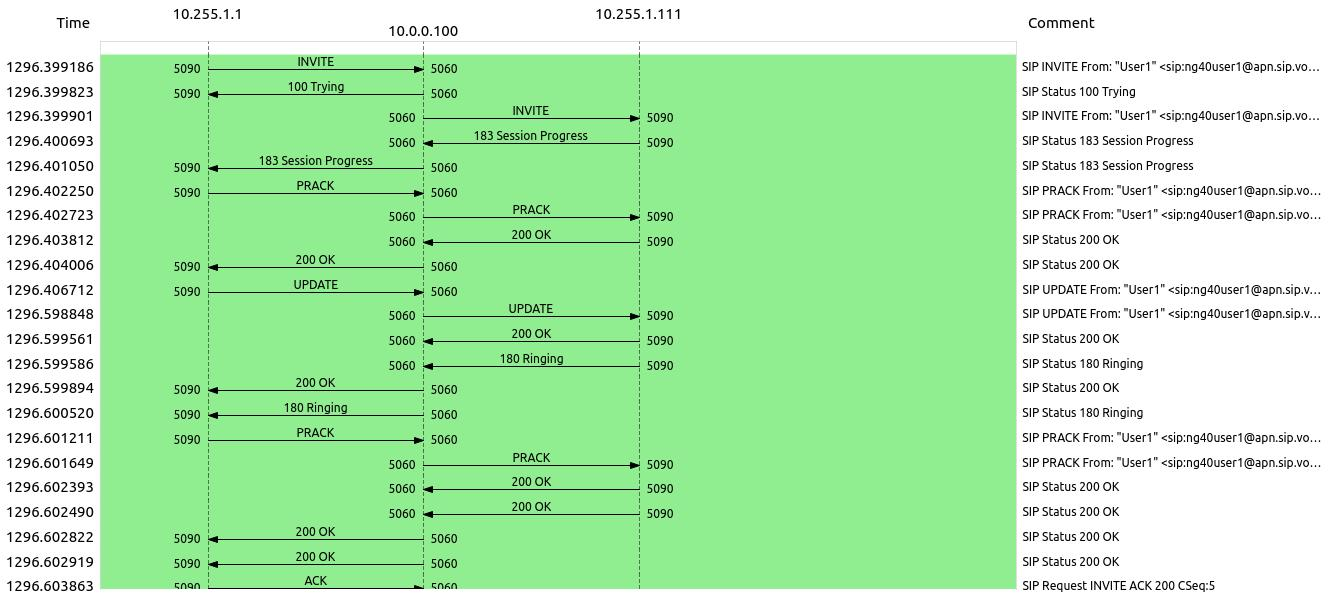
\includegraphics[scale=0.3]{images/call.jpg}
\end{center}

\textbf{b) Dibuja la torre de protocolos del paquete de datos de usuario que le llega al S-GW
incluyendo los protocolos de nivel de aplicación identificados en la pregunta anterior.}

\begin{center}
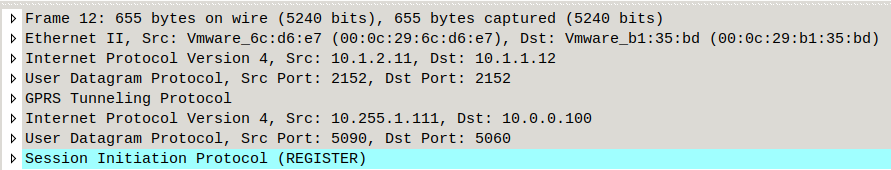
\includegraphics[scale=0.3]{images/protocolos.png}
\end{center}

En esta torre de protocolos se ve que por encima del User Datagram Protocol se encuentran GPRS Tunneling Protocol y otra vez Internet Protocol y ser Datagram Protocol porque al enviar los paquetes desde el dispositivo, se envían al eNodeB, que a su vez lo envía tunelado (por eso el protocolo GPRS Tunneling Protocol) a la central a través del protocolo Internet Protocol.

\textbf{c) ¿Cuál es la IP del UE? Indica si hay varios UEs involucrados en la comunicación y dé qué modo.}

Hay dos UE, ya que para una llamada se necesitan dos dispositivos. Sus IPs son 10.1.2.10 y 10.1.2.11.

\begin{center}
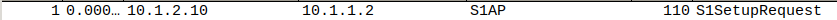
\includegraphics[scale=0.3]{images/UE1.png}
\end{center}

\begin{center}
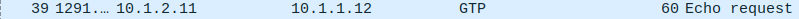
\includegraphics[scale=0.3]{images/UE2.png}
\end{center}

\textbf{d) ¿Cuál es la IP del eNodeB?}

Hay dos eNodeB, y sus IPs son 10.1.1.2 y 10.1.1.12.

\begin{center}
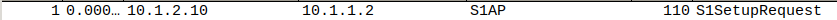
\includegraphics[scale=0.3]{images/UE1.png}
\end{center}

\begin{center}
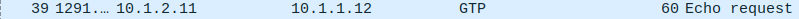
\includegraphics[scale=0.3]{images/UE2.png}
\end{center}

\textbf{e) ¿Cuál es la IP del S-GW?}

La dirección IP es 10.0.0.100.

\begin{center}
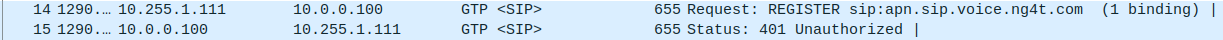
\includegraphics[scale=0.3]{images/SGW.png}
\end{center}

\section{Ejercicio 2. Traza handover.pcap}

\textbf{a) ¿Cuál es el id de la celda destino?}

10.200.20.254, ya que el primer mensaje está dirigido a la BTS.

\textbf{b) ¿Cuál es el id de la celda origen?}

10.200.10.37, ya que el primer mensaje es el dispositivo iniciando la conexión con la BTS.

\begin{center}
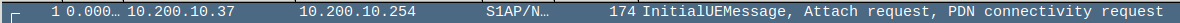
\includegraphics[scale=0.3]{images/celdaDestino.png} 
\end{center}

\textbf{c) ¿Cuándo se ejecuta el procedimiento de actualización de posición?}

Cuando el dispositivo envía un mensaje a la BTS inicial con una petición para cambiar de celda.

\begin{center}
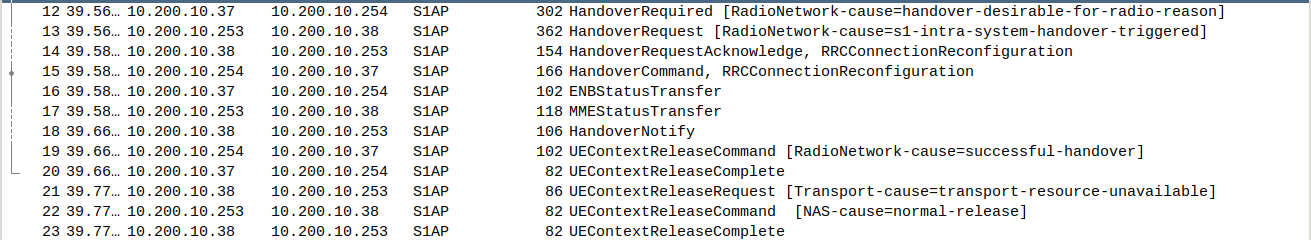
\includegraphics[scale=0.27]{images/handover.png} 
\end{center}

Tras esto, las direcciones IP quedan como sigue:

\begin{itemize}
\item \textbf{Dispositivo:} 10.200.10.38
\item \textbf{BTS:} 10.200.20.253
\end{itemize}

\end{document}